\documentclass{article}
\usepackage{amsmath, amssymb}
\usepackage[T1]{fontenc}
\usepackage[utf8]{inputenc}
\usepackage{lmodern}
\usepackage{graphicx}

\begin{document}

\begin{center}
\LARGE Informatik D Aufgabenblatt 1\\
\small Andrea Suckro, Sebastian Höffner
\end{center}
\vspace{0.3cm}
\normalsize

\section*{Aufgabe 1.1}

Sortierung der Funktionen nach $f_i\in\mathcal{O}(f_{i+1})$:

\begin{align*}
  \log(n) 
< \sqrt{n}
< \frac{n}{\sqrt{n}}
< n^{0.99}
< \frac{n}{\log(n)}
< \frac{n}{\log^2(n)}
< n                   
< n\log(n) \\
< n\log(n^2)
< n\log^2(n)           
< n^{1.01}
< 2^n 
< 2^{n+1}
< 2^{2n}
\end{align*}

\noindent Funktionen die auch in $\Theta(f_{i+1})$ liegen:\\ % moved ``liegen'' out of the math thing
$\sqrt{n},\ n \log(n),\ 2^n$

\section*{Aufgabe 1.2}

(a) Zeigen, dass $f_2 \in \mathcal{O}(f_1)$ f\"ur $c=1001,n_0=1$ gilt:
\begin{align*}
n^2+1000n &\leq cn^2 \\
1000n &\leq n^2(c - 1)\\
1000 &\leq n(c-1)\\
1000 &\leq 1000n, \forall n\geq n_0
\end{align*}

Alternative: $n^2+1000n\leq n^2+1000n^2 = 1001 n^2 \leq cn^2$

\noindent (b) Zeigen, dass $f_3 \in \mathcal{O}(f_4)$ liegt.
\begin{align*}
     m^{\log n}  &\leq      c\ n^{\log m}      \\
\log{\left(m^{\log n}\right)} &\leq \log{\left(c  n^{\log m}\right)}     \\
\log m  \log n   &\leq \log c  + \log n \log m \\
             0   &\leq \log c                    
\end{align*}
\noindent Da $c$ eine positive Konstante ist, ist die Gleichung erf\"ullt und $f_3 \in \mathcal{O}(f_4)$.

\noindent { }

\noindent (c) Zeigen, dass $f_6 \notin \mathcal{O}(f_5)$ liegt. 

Wir nehmen zun\"achst an $f_6$ liege in $\mathcal{O}(f_5)$. Dann existiert ein c, sodass ein $n_0$ existiert, f\"ur das alle $n \geq n_0$ gilt: $f_6(n)\leq cf_5(n)$. Nun existiert allerdings f\"ur jedes beliebige $n_0$ ein $n_1$, f\"ur das folgendes gilt: $n_1>n_0,n_1>100,n_1 =2k+1; n_1,k \in \mathbb{N}$. Wir setzen dieses in die gegebenen Formeln ein und erhalten f\"ur die Ungleichung:
\begin{align*}
n_1^3 &\leq cn_1 \\
n_1^2 &\leq c
\end{align*}
\noindent Es existieren in $\mathbb{N}$ nun beliebige weitere $n_{2...i}$ f\"ur die die Bedingungen von $n_1$ gelten und $n_2<n_3<...<n_i$. Die Ungleichung ist f\"ur ein konstantes c also nicht erf\"ullbar. $f_6$ kann also nicht in $\mathcal{O}(f_5)$ liegen.

\section*{Aufgabe 1.3}

\noindent (a) Aufz\"ahlung der Sprachen:
\begin{align*}
L_{min} &= \{aa,ab,ac,ca,ba\}\\
L_{max} &= \{ab,ba,bb,ac,ca,cc,bc,cb\}\\
L_{min}\cap L_{max} &= \{ab,ba,ac,ca\}\\
L_{min}\cup L_{max} &= \{aa,ab,ac,ba,ca,bb,bc,cc,cb\}\\
L_{min}\setminus L_{max} &= \{aa\}
\end{align*}

\noindent (b) Komplement der Sprache. $\overline{L_{min}}$:
$\left\{\epsilon, a, b, c, (b,c)^2, (a,b,c)^i | i\geq 3,i\in \mathbb{N}\right\} $

alternativ: $\{\epsilon\}\cup\{a,b,c\}\cup\{(b,c)^2\}\cup\Sigma^3\Sigma^*$

\noindent (c) $(L_{min} \setminus L_{max})^*=\left\{(aa)^i | i\geq 0,i\in \mathbb{N} \right\}$

\section*{Exercise 1.4}
\noindent (a) $\mathbb{L}=\left\{a^{2i+1}, b^{2j}: i,j \in \mathbb{N}, j\geq 1 \right\}$ 

oder alternativ: $\mathbb{L}=\left\{a^{2k+1}, k \in \mathbb{N} \right\} \cup \left\{b^{2k}, k \in \mathbb{N}^+ \right\}$

\noindent (b) $\mathbb{L} = \left\{ a^1 (ca)^i, i \in \mathbb{N} \right\} \cup \left\{ b^1 (ca)^i, i \in \mathbb{N} \right\}$

\noindent (c) $\mathbb{X} = \left\{aba,bab,abb\right\}$ für $\bigcup\limits_{i=1}^{\infty} \mathbb{X}_{j=1}^i\mathbb{X}$ oder $\mathbb{L} = \left\{x_1x_2x_3...x_n: x_i \in \mathbb{X}, n \in \mathbb{N}^+\right\}$

\section*{Exercise 1.6}

Wir kodieren die  :) = (s)mile, :| = (n)eutral, :( = (f)rown.

\noindent (a) Grammatik f\"ur alle W\"orter die mit ss beginnen und mit ff aufh\"oren.
\begin{align*}
S &\rightarrow\ sA\\
A &\rightarrow\ sB\\
B &\rightarrow\ sB\ |\ nB\ |\ fB\ |\ fE\\
E &\rightarrow\ f\ %|\ sB\ |\ nB
\end{align*}

\noindent (b) Grammatik f\"ur alle W\"orter mit mindestens drei mal nn.
\begin{align*}
S &\rightarrow\ nA\ |\ sS\ |\ fS\\
A &\rightarrow\ nB\ |\ sS\ |\ fS\\
B &\rightarrow\ nC\ |\ sB\ |\ fB\\
C &\rightarrow\ nD\ |\ sB\ |\ fB\\
D &\rightarrow\ nE\ |\ sD\ |\ fD\\
E &\rightarrow\ n\ |\ nF\ |\ sD\ |\ fD\\
F &\rightarrow\ s\ |\ f\ |\ n\ |\ sF\ |\ fF\ |\ nF
\end{align*}

\noindent (c) Grammatik f\"ur genau zwei mal ss.
\begin{align*}
S &\rightarrow\ sA\ |\ fS\ |\ nS\\
A &\rightarrow\ sB\ |\ fS\ |\ nS\\
B &\rightarrow\ fC\ |\ nC\\
C &\rightarrow\ sD\ |\ fC\ |\ nC\\
D &\rightarrow\ sE\ |\ fC\ |\ nC\ |\ s\\
E &\rightarrow\ f\ |\ n\ |\ fF\ |\ nF\\
F &\rightarrow\ s\ |\ f\ |\ n\ |\ fF\ |\ nF\ |\ sE
\end{align*}

% habe ex 1.5 ans Ende geschoben, passt besser denke ich
\section*{Exercise 1.5}
\begin{figure}[ht]
 \centering
 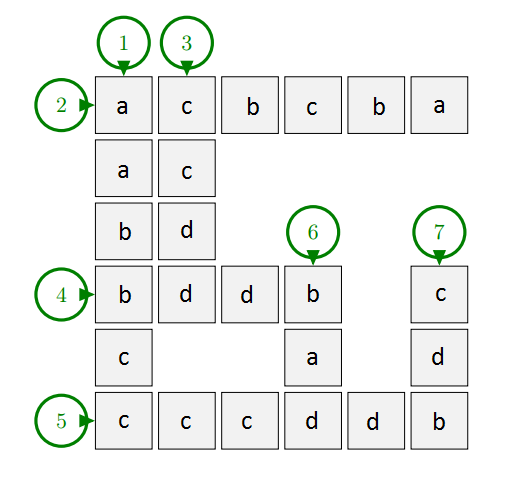
\includegraphics[scale=0.5]{KreuzwortRaetsel.png}
 \caption{L\"osung}
 \label{figure1}
\end{figure}

\end{document}